\cleardoublepage
\chapter{Video Coding Transforms}

%%%%%%%%%%%%%%%%%%%%%%%%%%%%%%%%%%%%%%%%%%%%%%%%%%%%%%%%%%%%%%%%%%%%%%%%%%%%%%
\section{{Introduction}}

\textcolor{red}{As mentioned previously,} the basic principle behind the compression of video, is the reduction of inter-pixel/inter-symbol correlation. The various integral blocks of a video compression system try to accomplish this objective through different strategies. The \emph{Intra-frame} and \emph{Inter-frame Prediction} exploit spatial and temporal correlation, respectively. Through the subtraction of the input by the output of one of these blocks, and the attainment of the \emph{residue}, the next compression stage is made in the \emph{Transform} block
\todo{as seen in ...}
,which is the focus of this work.

\todo[inline,color=red!40]{Verify accordance with previous chapter}

The technique implemented by this process relies on the energy compaction in the frequency domain to reduce the correlation within a frame block, i.e. the input of the Transform block is evaluated on its main frequencies --- the \emph{transform coefficients} --- on a spatial and/or temporal domain, similarly to the process executed on an \gls{fft}. Once each block is quantized on these coefficients, the compression is made with the removal of the least significant ones, on the \emph{Quantization} stage. The intent of the \emph{transform} is to split the image into a set of predefined coefficients, that get transmitted instead of the pixel values.

The objective of this chapter is to give the reader a basic understanding of the theoretical basis behind said Transformations, as well as to introduce the most commonly used ones. 

%%%%%%%%%%%%%%%%%%%%%%%%%%%%%%%%%%%%%%%%%%%%%%%%%%%%%%%%%%%%%%%%%%%%%%%%%%%%%%
\section{Background}
%%%%%%%%%%%%%%%%%%%%%%%%%%%%%%%%%%%%%%%
\subsection{Basis vector/image interpretation}

A useful interpretation, and a good starting point to the study of this process, is to see it as the decomposition of the input as a set of basis vectors (1D transforms) or images/matrices (2D transforms). The transformation outputs , $T_i$, can be seen as the weights of each basis vector/image, $\vec{e_i}$, that summed return the input, $\vec{g}$, i.e.

\begin{equation}
    \vec{g} = \sum_{i=1}^{N} T_i \vec{e_i}
\end{equation}
which means that the coefficients are related to the amount of correlation between the input and each basis component, and can be obtained with the \emph{inner product} of the input and each basis vector.

\begin{equation} \label{eq:coef_vec}
    T_i = \vec{e_i}^T \vec{g}
\end{equation}

Since each input vector will have different correlation values between the various basis vectors, this operation accomplishes two main objectives:

\begin{itemize}
    \item De-correlation of the input values
    \item Signaling of the most important basis vectors.
\end{itemize}

Considering a 2D image, $g(x,y)$, and its corresponding transformed coefficients, $T(u,v)$, where $(x,y)$ are the pixel coordinates, and $(u,v)$ are the corresponding coordinates in the transform domain, we can obtain an analogous version of equation \ref{eq:coef_vec} as

\begin{equation} \label{eq:Tmatsum}
    T(u,v) = \sum_{x=0}^{M-1}\sum_{y=0}^{N-1}g(x,y)f(x,y,u,v)
\end{equation}

Similarly, we can re-obtain the original picture

\begin{equation} \label{eq:Gmatsum}
    g(x,y) = \sum_{u=0}^{M-1}\sum_{v=0}^{N-1}T(u,v)i(x,y,u,v)
\end{equation}
where $f(x,y,u,v)$ and $i(x,y,u,v)$ are the \emph{forward} and \emph{inverse transformation kernels}. To better explain the concept of these, first it's needed to introduce the two following concepts.

%%%%%%%%%%%%%%%%%%%%%%%%%%%%%%%%%%%%%%%%%%%
% ATTENTION: "BETTER EXPLAIN ... FIRST IT'S NEEDED" gives the idea that there is going to be a later explanation
%%%%%%%%%%%%%%%%%%%%%%%%%%%%%%%%%%%%%%%%%%%

%%%%%%%%%%%%%%%%%%%
\subsubsection{Separability}

A useful characteristic of 2D Video Coding Transforms is its ability to be independently calculated between rows and columns. This means that given a 2D block as input, the transform coefficients can be calculated first with the \emph{horizontal transform}, and then with the \emph{vertical transform}, or vice-versa.

This aspect is applicable if the following conditions are applied

\begin{equation} \label{eq:fwf1f2}
    f(x,y,u,v)=f_1(x,u)f_2(y,v)
\end{equation}


\begin{equation} \label{eq:ini1i2}
    i(x,y,u,v)=i_1(x,u)i_2(y,v)
\end{equation}

This means that the equation \ref{eq:Tmatsum} is reconstructed as 2 independent and sequential operations

\begin{gather}
    T_{temp}(x,v) = \sum_{y=0}^{N-1}g(x,y)f_2(y,v) \\
    T(u,v) = \sum_{x=0}^{M-1}T_{temp}(x,v)f_1(x,u)
\end{gather}

On AV1, due to the various implemented transformation kernels, this aspect is severely explored, since the only way of implementing the combination of different 1D kernels, is to calculate them independently. This aspect is further explained with the following concept.

%%%%%%%%%%%%%%%%%%%
\subsubsection{Symmetry}

Taking equation \ref{eq:fwf1f2}, a transformation kernel is said to be symmetric if 

\begin{equation}
    f_1(y,v) = f_2(x,u)
\end{equation}

This characteristic is particularly useful because it makes the forward and inverse transformations expressible as matrix multiplications. Therefore, the equations \ref{eq:Tmatsum} and \ref{eq:Gmatsum} are represented, respectively, as

\begin{equation}
    T = F^TGF 
\end{equation}
\begin{equation}
    G = I^TTI
\end{equation}
where $F$ and $I$ are the forward and inverse transform matrices. This aspect is only possible for square matrix, i.e., input blocks with the same height and width.

\textcolor{red}{This concept isn't exploited in AV1, since the use of different 1D transformation kernels, and rectangular block sizes ($M \neq N$) make the 2D transform asymmetric, and therefore, not executable as matrix multiplication.}

\textsep

Looking now at equation \ref{eq:Gmatsum}, we can interpret the inverse transformation kernel as a set of basis images, dependent of the $(u,v)$ pair. By this, it is meant 

\begin{equation}
    g(x,y) = \sum_{u=0}^{M-1}\sum_{v=0}^{N-1}T(u,v)I_{u,v}
\end{equation}
where

\begin{equation}
    I_{u,v}=\begin{bmatrix}
                i(0,0,u,v) & i(0,1,u,v) & \dots & i(0,M-1,u,v) \\
                i(1,0,u,v) & i(1,1,u,v) & \dots & i(1,M-1,u,v) \\
                \vdots     & \vdots     & \dots & \vdots       \\
                i(N-1,0,u,v) & i(N-1,1,u,v) & \dots & i(N-1,M-1,u,v) \\
            \end{bmatrix}
\end{equation}

Therefore, the forward and inverse transformation process can be seen as the deconstruction of an input block, into a set of $M \cdot N$ basis images, dependent of the used transformation kernel. As expressed in equations \ref{eq:fwf1f2} and \ref{eq:ini1i2}, this analogy can be made on a 1D space \nocite{shiImageVideoCompression2008}.

\todo[inline,color=red!40]{JPEG example?}

Given a general comprehension of the theoretical principles behind the \emph{Transform} block, now the most common transformation kernels are introduced, with focus on the AV1 video codec.

%%%%%%%%%%%%%%%%%%%%%%%%%%%%%%%%%%%%%%%%%%%%%%%%%%%%%%%%%%%%%%%%%%%%%%%%%%%%%%
\section{Transformation Kernels}
%%%%%%%%%%%%%%%%%%%%%%%%%%%%%%%%%%%%%%%
\subsection{Discrete Fourier Transform (DFT)}

Although it isn't implemented in video coding, it's widely used in digital signal processing, and many of the used transformation kernels are approximations of this function.

It has it's roots on the \emph{Fourier Transform}, whose forward and inverse transformations are expressed in equations \ref{eq:fourf} and \ref{eq:fouri}, respectively.

\begin{equation} \label{eq:fourf}
    T(u,v) = \int_{-\infty}^{\infty}\int_{-\infty}^{\infty}g(x,y)e^{-j2\pi(ux+vy)} dx \, dy
\end{equation}

\begin{equation} \label{eq:fouri}
    g(x,y) = \int_{-\infty}^{\infty}\int_{-\infty}^{\infty}T(u,v)e^{j2\pi(ux+vy)} du \, dv
\end{equation}

Once we consider a finite number of points, the previous equations become

\begin{equation} \label{eq:dftf}
    T(u,v) = \frac{1}{MN}\sum_{x=0}^{M-1}\sum_{y=0}^{N-1}g(x,y)e^{-j2\pi \left(\frac{ux}{M}+\frac{vy}{N}\right)}
\end{equation}

\begin{equation} \label{eq:dfti}
    g(x,y) = \sum_{u=0}^{M-1}\sum_{v=0}^{N-1}T(u,v)e^{j2\pi \left(\frac{ux}{M}+\frac{vy}{N}\right)}
\end{equation}
which corresponds to replacing the kernels in equations \ref{eq:Tmatsum} and \ref{eq:Gmatsum} with

\begin{gather}
    f(x,y,u,v) = \frac{1}{MN} e^{-j2\pi \left(\frac{ux}{M}+\frac{vy}{N}\right)} \\
    i(x,y,u,v) = e^{j2\pi \left(\frac{ux}{M}+\frac{vy}{N}\right)}
\end{gather}

The position of the multiplication factor, $\frac{1}{MN}$, is irrelevant, and in some works is divided into two terms in the forward and inverse kernels, $\frac{1}{M}$ and $\frac{1}{N}$, or even $\frac{1}{\sqrt{MN}}$. \nocite{gonzalezDigitalImageProcessing2018}

Because of the use of complex numbers, this operation tends require a high computational effort, whence its disuse in video coding.

%%%%%%%%%%%%%%%%%%%%%%%%%%%%%%%%%%%%%%%
\subsection{Discrete Walsh-Hadamard Transform (WHT)}

This transformation replaces the sum of sines and cosines of the DFT, alternating of positive and negative $1$'s, depending on the binary representation of the inputs.

Considering the inputs of the transform to be represented with $m$ bits, where $m-1$ is the most significant bit ($b_{m-1}$), the forward and inverse kernels are represented as

\begin{equation}
    f(x,y,u,v) = i(x,y,u,v) = \frac{1}{\sqrt{MN}}(-1)^{\sum_{i=0}^{m-1}\lfloor b_i(x)p_i(u)+b_i(y)p_i(v)\rfloor}
\end{equation}
where

\begin{align*}
    &p_0(u)=b_{m-1}(u) \\
    &p_1(u)=b_{m-1}(u) +b_{m-2}(u) \\
    \,&\vdots \addtocounter{equation}{1}\tag{\theequation} \\
    &p_{m-1}(u)=b_1(u)+b_0(u) 
\end{align*}

%%%%%%%%%%%%%%%%%%%%%%%%%%%%%%%%%%%%%%%
\subsection{Discrete Cosine Transform (DCT)}

The most commonly used transform, the \emph{DCT}, was published by Ahmed et al. in 1974 \cite{ahmedDiscreteCosineTransform1974}. Since then, it has been adopted in a wide range of applications, being the only transform used in the first generations of video codecs, as well as in \emph{still image compression}, being the basis of the \emph{\gls{JPEG}} standard.

It is frequently compared to the \emph{DFT}, due to the similarity of their operation. However, as the name implies, the \emph{DCT} relies on the cosine function to create its basis images, which is a \emph{periodic} and \emph{symmetrically even} function. Therefore, as mentioned by \cite[A. V. Oppenheim]{oppenheimDiscretetimeSignalProcessing1998}, \emph{"Just as the DFT involves an implicit assumption of periodicity, the DCT involves implicit assumptions of both periodicity and even symmetry"}.  This is easily observable once considered the equivalent process of both algorithms. Taking an $N$-point sequence, $g(n)$, the calculation of the \emph{DFT} and \emph{DCT} of such sequence is equivalent to the processes presented at table \ref{tab:DFTDCT}.

\begin{table}[h]
    \centering
    \begin{tabular}{l|r|r|r|r} 
        \textbf{Step} &      \multicolumn{2}{r|}{\textbf{\emph{DFT}}} &      \multicolumn{2}{r}{\textbf{\emph{DCT}}} \\ \hline
        1 &         \multicolumn{2}{p{0.4\textwidth}|}{Repeat $g(n)$ every N points, giving origin to $\widetilde{g}_N(n)$} &         \multicolumn{2}{p{0.4\textwidth}}{Concatenate $g(n)$ with a flipped version of itself, creating a $2N$ sequence, $g_{2N}(n)$, and repeat it, giving origin to $\widetilde{g}_{2N}(n)$}\\ \hline
        2 &         \multicolumn{2}{p{0.4\textwidth}|}{Calculate the \emph{Fourier} expansion of $\widetilde{g}_N$} &         \multicolumn{2}{p{0.4\textwidth}}{Calculate the \emph{Fourier} expansion of $\widetilde{g}_{2N}$}\\ \hline
        3 &         \multicolumn{2}{p{0.4\textwidth}|}{Keep the first $N$ coefficients\, and set all others to $0$} &         \multicolumn{2}{p{0.4\textwidth}}{Keep the first $N$ coefficients, and set all others to $0$}\\ 
    \end{tabular}
    \caption{Similarity between the processes of the        \emph{DFT} and the \emph{DCT}}
    \label{tab:DFTDCT}
\end{table}

The main reason behind the heavy adoption of the \emph{DCT} is its great energy compaction on the lower frequencies, where most of the energy in a picture is packed. If the the output of the first step of table \ref{tab:DFTDCT} is observed, this aspect is more easily understood.

Due to the back-to-head repetition seen in figure \ref{subfig:dft2n}, there is a disruption every $N$ points, which gives origin to high frequency components in the \emph{Fourier} transform. Therefore, the more continuous behavior obtained with the back-to-back repetition of the \emph{DCT} gives origin to more significant low frequency coefficients. However, there are many ways of creating a periodic and symmetric sequence from a finite number of points. This factor has led to the implementation of different versions of the \emph{DCT}, which differ in minor details between themselves. These differences are consequence of the way the symmetry is obtained, which can be observed in figure \ref{subfig:dct2n}. The represented implementations are referred to as \emph{DCT-1} to \emph{DCT-4}, but other possibilities exist.

\begin{figure}[h]
    \centering 
        \begin{subfigure}[c]{\textwidth}
            \centering
            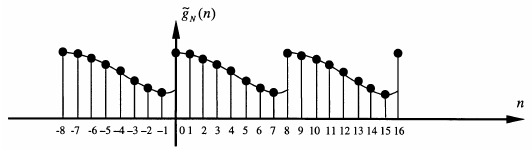
\includegraphics[width=0.8\textwidth]{Sections/3Transforms/Images/DFT2N.png}
            \caption{\emph{DFT}}
            \label{subfig:dft2n}
        \end{subfigure}
        \begin{subfigure}[c]{\textwidth}
            \centering
            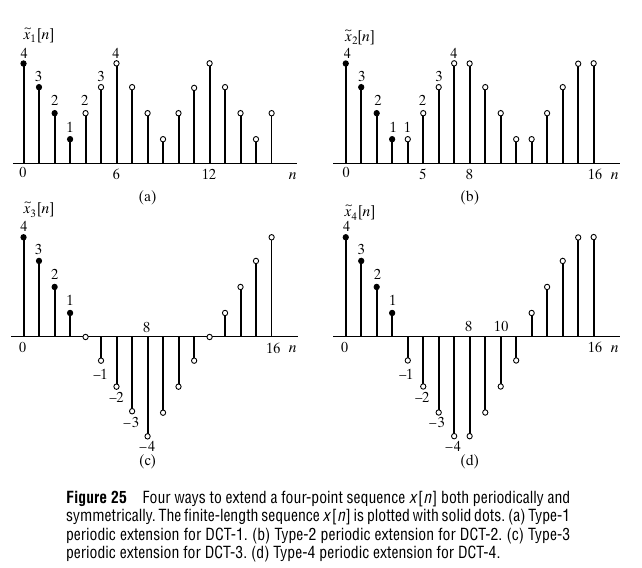
\includegraphics[width=0.8\textwidth]{Sections/3Transforms/Images/DCTs2N.png}
            \caption{\emph{DCT}}
            \label{subfig:dct2n}
        \end{subfigure}
    \caption[Sequences generated in the first step of table \ref{tab:DFTDCT}]{Sequences generated in the first step of table \ref{tab:DFTDCT} \cite{shiImageVideoCompression2008}}
    \label{fig:2NSeq}
\end{figure}
\todo[inline]{Change image to TIKZ}

Of the different implementations, \emph{DCT-1} and \emph{DCT-2} are the most commonly used, being the \textcolor{red}{focus of this work}. 

\subsubsection{}

\printbibliography[heading=subbibliography]
\addcontentsline{toc}{section}{References}